% !TeX root = construct.tex

\selectlanguage{hebrew}

\chapter{איך לרבע את המעגל )בערך(}\label{c.square-a-circle}


\section{%
קירובים ל-%
$\pi$}

היוונים חקרו בנייה גיאומרטית עם סרגל ומחוגה. הם לא הצליחו לפתור שלוש בעיות: חלוקת זווית לשלושה חלקים שווים, הכפלת קוביה )נתונה קוביה, בנה קוביה בנפח פי-שניים(, וריבוע מעגל )נתון מעגל, בנה ריבוע עם אותו שטח(. במאה ה-%
$19$
הוכח שאין פתרונות לבעיות אלו.

אם נתונה קטע קו שאורכו
$1$,
המספרים )אורכי הקטעים( שניתן לבנות מהקטע הזה הם התוצאות של חישובים עם פעולות החשבון
$+,-,\times,\div,\surd$.
לא ניתן להכפיל קוביה: הבנייה מחייבת לפתור את המשוואה
$x^3-2=0$
ולבנות את האורך
$\sqrt[3]{2}$,
אבל אי-אפשר לבנות קטע שהוא שורש שלישי של קטע נתון. מאותה סיבה לא ניתן לחלק זווית לשלושה, כי כדי לחלק 
$60^\circ$
לשלושה חלקים, חייבים לפתור את המשוואה 
$8x^3-6x-1=0$.

רק בשנת
$1882$
הוכח שאי-אפשר לרבע מעגל. נתון מעגל יחידה ששטחו
$\pi 1^2=\pi$,
יש לבנות ריבוע שהצלע שלו באורך
$\sqrt{\pi}$.
אבל
$\pi$
הוא מספר
\textbf{טרנסנדנטלי},
מספר אינו פתרון של אף משוואה אלגבראית. ההוכחה מסובכת ביותר ומשתמשת במושגים מאנליזה.

קיימים קירובים פשוטים ל-%
$\pi$,
למשל:
\[
\frac{355}{113}=3.14159292\,,
\]
שההפרש בינו לבין
$\pi\approx 3.14159265$
הוא רק 
$2.67\times 10^{-7}$.
רדיוס כדור הארץ הוא בערך
$6,378.1$
ק"מ. חישוב ההיקף עם
$355/113$
נותן תוצאה של
$40,074.78421$
ק"מ וחישוב עם
$\pi$
נותן תוצאה של
$40,074.78761$
ק"מ. ההפרש הוא פחות מ-%
$4$
מטר!

ניתן לבנות כל מספר הרציונלי. העתיק את הקטע באורך 
$1$
לפי המספר במונה ולפי המספר במכנה, ובנה את הקטע באורך החילוק ביניהם )הבנייה מסתמכת על משפט תאלס(. כאן נביא בנייה קצרה של קטע קו באורך
$355/113$
מאת רמנוג'ן
\L{Ramanujan}
\L{\cite{ramanujan}}.
נציג את הבנייה בשלבים כאשר חלק מהבנייה וההוכחה מוצג כתרגילים. את התשובות ניתן למצוא בסוף הפרק.

רמנוג'ן
\L{(1887--1920)}
גדל בדרום הודו. מהר מאוד הוא התקדם מעבר לרמה של בתי הספר המקומיים. הוא שלח את עבודותיו למתמטיקאי האנגלי
\L{G.H. Hardy}
שהזמין אותו לאנגליה. רמנוג'ן הגיע בשנת
$1914$,
וחזרתו להודו לא התאפשרה עד לסיום מלחמת העולם הראשונה. הוא סבל רבות ממזג האוויר הקר ומהאוכל הלא מוכר. הוא היה צמחוני בניגוד לאנגלים באותה תקופה באכלו הרבה אוכל מהחי: בשר, חלב, ביצים. זמן קצר לאחר שובו להודו נפטר בגיל 
$32$.
המתמטיקה שהגה רמנוג'ן נחקרת עד היום. לפרטים על חייו של רמנוג'ן ראו
\L{\cite{kanigel}}.



\np

%%%%%%%%%%%%%%%%%      First

\begin{center}
\textbf{\Large שלב 1}
\end{center}

\begin{itemize}
\item
בנה מעגל יחידה עם מרכז
$O$
וקוטר
$PR$.
\item 
סמן
$H$
במחצית הקטע
$PO$,
וסמן
$T$
כשליש הקטע
$RO$.
\item
בנה אנך מ-%
$T$
שחותך את המעגל ב-%
$Q$.
\item 
בנה מיתר
$RS$
שאורכו שווה ל-%
$QT$.
\end{itemize}

\begin{center}
\selectlanguage{english}
\begin{tikzpicture}[scale=.9]
\clip (-5.5,-5.1) rectangle +(11,10.2);
% Draw circle and horizontal diameter
\draw[name path=circle] (0,0)  coordinate (o) node[below] {$O$} circle[radius=5cm];
\draw (-5,0) coordinate (p) node[left] {$P$} -- (5,0) coordinate (r) node[right] {$R$};
\fill (o) circle (1pt);
\fill (p) circle (1pt);
\fill (r) circle (1pt);
\fill (-2.5,0) coordinate (h) node[below] {$H$} circle (1pt);
\fill (10/3,0) coordinate (t) node[below] {$T$} circle (1pt);
\path (p) -- node[above,xshift=12pt] {$1/2$} (h) -- node[above] {$1/2$} (o) -- node[above] {$2/3$} (t) -- node[above] {$1/3$} (r);
% Draw perpendicular TQ
\path[name path=tq] (t) -- +(0,5);
\path[name intersections={of=tq and circle,by=q}];
\draw (t) -- node[left] {$a$} (q) node[above] {$Q$};
\fill (q) circle (1pt);
% Draw chord RS
\path[name path=rcirc] (r) let \p1 = ($ (t) - (q) $) in circle ({veclen(\x1,\y1)});
\path[name intersections={of=rcirc and circle,by=s}];
\draw (r) -- node[left] {$a$} (s);
\fill (s) node[above right] {$S$} circle (1pt);
\draw (p) -- node[above] {$b$} (s);
\end{tikzpicture}
\end{center}

\exer{}
בנה את האורך 
$TR=\disfrac{1}{3}$.

\exer
חשב את אורכו של
$QT$.

\exer
חשב את אורכו של
$PS$.

\exer
בנה את המיתר
$RS$
שאורכו שווה ל-%
$QT$.

\np

%%%%%%%%%%%%%%%%%      Second

\begin{center}
\textbf{\Large שלב 2}
\end{center}

\begin{itemize}
\item 
בנה קטעי קו
$NT$
ו-%
$OM$
מקביליים ל-%
$RS$.
\end{itemize}

\begin{center}
\selectlanguage{english}
\begin{tikzpicture}[scale=.9]
\clip (-5.5,-5.1) rectangle +(11,10.2);
% Draw circle and horizontal diameter
\draw[name path=circle] (0,0)  coordinate (o) node[below] {$O$} circle[radius=5cm];
\draw (-5,0) coordinate (p) node[left] {$P$} -- (5,0) coordinate (r) node[right] {$R$};
\fill (o) circle (1pt);
\fill (p) circle (1pt);
\fill (r) circle (1pt);
\fill (-2.5,0) coordinate (h) node[below] {$H$} circle (1pt);
\fill (10/3,0) coordinate (t) node[below] {$T$} circle (1pt);
% Draw chord RS and line PS
\path[name path=tq] (t) -- +(0,5);
\path[name intersections={of=tq and circle,by=q}];
\path[name path=rcirc] (r) let \p1 = ($ (t) - (q) $) in circle ({veclen(\x1,\y1)});
\path[name intersections={of=rcirc and circle,by=s}];
\draw (r) -- node[left] {$a$} (s);
\fill (s) node[above right] {$S$} circle (1pt);
\draw[name path=ps] (p) -- node[above right,xshift=8pt,yshift=8pt] {$b$} (s);
% Draw TN
\path[name path=tn] (t) -- +($(s)-(r)$);
\path[name intersections={of=ps and tn,by=n}];
\draw (t) -- (n);
\fill (n) node[above] {$N$} circle (1pt);
% Draw OM
\path[name path=om] (o) -- +($(s)-(r)$);
\path[name intersections={of=ps and om,by=m}];
\draw (o) -- (m);
\fill (m) node[above left] {$M$} circle (1pt);
% Label PM and MN
\path (p) -- node[below,xshift=12pt,yshift=4pt] {$c$} (m);
\path (m) -- node[below,xshift=8pt,yshift=4pt] {$d$} (n);
\end{tikzpicture}
\end{center}

\exer
חשב את אורכו של
$PM$.

\exer
חשב את אורכו של
$MN$.

\np

%%%%%%%%%%%%%%%%%      Third

\begin{center}
\textbf{\Large שלב 3}
\end{center}


\begin{itemize}
\item
בנה את המיתר
$PK=PM$.
\item
בנה את המשיק
$PL=MN$.
\item 
חבר את הנקודות
$K,L,R$.
\end{itemize}

\begin{center}
\selectlanguage{english}
\begin{tikzpicture}[scale=.9]
\clip (-5.5,-5.1) rectangle +(11,10.2);
% Draw circle and horizontal diameter
\draw[name path=circle] (0,0)  coordinate (o) node[below] {$O$} circle[radius=5cm];
\draw (-5,0) coordinate (p) node[left] {$P$} -- (5,0) coordinate (r) node[right] {$R$};
\fill (o) circle (1pt);
\fill (p) circle (1pt);
\fill (r) circle (1pt);
\fill (-2.5,0) coordinate (h) node[below] {$H$} circle (1pt);
\fill (10/3,0) coordinate (t) node[below] {$T$} circle (1pt);
% Draw chord RS and line PS
\path[name path=tq] (t) -- +(0,5);
\path[name intersections={of=tq and circle,by=q}];
\path[name path=rcirc] (r) let \p1 = ($ (t) - (q) $) in circle ({veclen(\x1,\y1)});
\path[name intersections={of=rcirc and circle,by=s}];
\draw (r) -- (s);
\fill (s) node[above right] {$S$} circle (1pt);
\draw[name path=ps] (p) -- (s);
% Draw TN
\path[name path=tn] (t) -- +($(s)-(r)$);
\path[name intersections={of=ps and tn,by=n}];
\draw (t) -- (n);
\fill (n) node[above] {$N$} circle (1pt);
% Draw OM
\path[name path=om] (o) -- +($(s)-(r)$);
\path[name intersections={of=ps and om,by=m}];
\draw (o) -- (m);
\fill (m) node[above left] {$M$} circle (1pt);
\path (p) -- node[below,xshift=12pt,yshift=4pt] {$c$} (m);
\path (m) -- node[below,xshift=8pt,yshift=4pt] {$d$} (n);
% Draw chord PK
\path[name path=pkcirc] (p) let \p1 = ($ (p) - (m) $) in circle ({veclen(\x1,\y1)});
\path[name intersections={of=pkcirc and circle,by={k1,k}}];
\draw (p) -- node[right,xshift=-2pt,yshift=10pt] {$c$} (k) node[below left] {$K$};
% Draw tangent PL
\draw let \p1 = ($ (m) - (n) $), \n1 = {veclen(\x1,\y1)} in (p) -- node[left] {$d$} (-5,-\n1) coordinate (l) node[left] {$L$};
% Connect L and K to R
\draw (r) -- node[above] {$f$} (l) -- (k) -- node[below right] {$e$} cycle;
\end{tikzpicture}
\end{center}

\exer
מה ידוע על 
$\triangle PKR$?
חשב את אורכו של
$RK$.

\exer
מה ידוע על
$\triangle PLR$?
חשב את אורכו של
$RL$.

\np

%%%%%%%%%%%%%%%%%      Fourth

\begin{center}
\textbf{\Large שלב 4}
\end{center}

\begin{itemize}
\item
סמן את הנקודה
$C$
כך ש-%
$RC=RH$.
\item 
בנה
$CD$
מקביל ל-%
$LK$.
\end{itemize}

\begin{center}
\selectlanguage{english}
\begin{tikzpicture}[scale=.9]
\clip (-5.5,-5.1) rectangle +(11,10.2);
% Draw circle and horizontal diameter
\draw[name path=circle] (0,0)  coordinate (o) node[below] {$O$} circle[radius=5cm];
\draw (-5,0) coordinate (p) node[left] {$P$} -- (5,0) coordinate (r) node[right] {$R$};
\fill (o) circle (1pt);
\fill (p) circle (1pt);
\fill (r) circle (1pt);
\fill (-2.5,0) coordinate (h) node[below] {$H$} circle (1pt);
% Get values of PM and MN but don't draw
\coordinate (t) at (10/3,0);
\path[name path=tq] (t) -- +(0,5);
\path[name intersections={of=tq and circle,by=q}];
\path[name path=rcirc] (r) let \p1 = ($ (t) - (q) $) in circle ({veclen(\x1,\y1)});
\path[name intersections={of=rcirc and circle,by=s}];
\path[name path=ps] (p) -- (s);
\path[name path=tn] (t) -- +($(s)-(r)$);
\path[name intersections={of=ps and tn,by=n}];
\path[name path=om] (o) -- +($(s)-(r)$);
\path[name intersections={of=ps and om,by=m}];
% Draw chord PK
\path[name path=pkcirc] (p) let \p1 = ($ (p) - (m) $) in circle ({veclen(\x1,\y1)});
\path[name intersections={of=pkcirc and circle,by={k1,k}}];
\draw (p) -- (k) node[below left] {$K$};
% Draw tangent PL
\draw let \p1 = ($ (m) - (n) $), \n1 = {veclen(\x1,\y1)} in (p) -- (-5,-\n1) coordinate (l) node[left] {$L$};
% Connect L and K to R
\draw (r) -- node[above] {$f$} (l) -- (k) -- node[below right] {$e$} cycle;
% Find point C on RK
\coordinate (c) at ($(r)!7.5cm!(k)$);
\path (r) -- node[above, near end] {$g$} (c);
\fill (c) node[below] {$C$} circle (1pt);
% Draw CD
\path[name path=cd] (c) -- +($(l)-(k)$);
\path[name path=lr] (l) -- (r);
\path[name intersections={of=cd and lr,by=d}];
\draw (c) -- (d);
\fill (d) node[above,xshift=2pt] {$D$} circle (1pt);
\path (r) -- node[below,near end] {$h$} (d);
\end{tikzpicture}
\end{center}


\exer
חשב את אורכו של
$RC$.

\exer
חשב את אורכו של
$RD$.

\exer
בנה ריבוע שאורך הצלע שלו הוא
$RD$.

\exer
חשב את
$RD^2$
שהוא שטח הריבוע. חשב גם כשבר וגם כמספר עשרוני.

\np

%%%%%%%%%%%%%%%%%      Fifth

\begin{center}
\textbf{\Large סיכום}
\end{center}

להלן הבנייה בשלמותה כאשר כל האורכים מסומנים.

\bigskip

\bigskip
\bigskip

\begin{center}
\selectlanguage{english}
\begin{tikzpicture}[scale=1.2,align=left]
\clip(-6,-5.1) rectangle +(11.5,10.2);
% Draw circle and horizontal diameter
\draw[name path=circle] (0,0)  coordinate (o) node[below] {$O$} circle[radius=5cm];
\draw (-5,0) coordinate (p) node[left] {$P$} -- (5,0) coordinate (r) node[right] {$R$};
\fill (o) circle (1pt);
\fill (p) circle (1pt);
\fill (r) circle (1pt);
\fill (-2.5,0) coordinate (h) node[below] {$H$} circle (1pt);
\fill (10/3,0) coordinate (t) node[below] {$T$} circle (1pt);
\path (p) -- node[above,xshift=10pt] {$1/2$} (h) -- node[above] {$1/2$} (o) -- node[above] {$2/3$} (t) -- node[above] {$1/3$} (r);
% Draw chord RS and line PS
\path[name path=tq] (t) -- +(0,5);
\path[name intersections={of=tq and circle,by=q}];
\path[name path=rcirc] (r) let \p1 = ($ (t) - (q) $) in circle ({veclen(\x1,\y1)});
\path[name intersections={of=rcirc and circle,by=s}];
\draw (r) -- node[left] {$\sqrt{5}/3$} (s);
\fill (s) node[above right] {$S$} circle (1pt);
\draw[name path=ps] (p) -- node[above right,yshift=16pt] {$\sqrt{31}/3$} (s);
% Draw TN
\path[name path=tn] (t) -- +($(s)-(r)$);
\path[name intersections={of=ps and tn,by=n}];
\draw (t) -- (n);
\fill (n) node[above] {$N$} circle (1pt);
% Draw OM
\path[name path=om] (o) -- +($(s)-(r)$);
\path[name intersections={of=ps and om,by=m}];
\draw (o) -- (m);
\fill (m) node[above left] {$M$} circle (1pt);
\path (p) -- node[below,xshift=32pt,yshift=12pt] {$\sqrt{31}/6$} (m);
\path (m) -- node[below,xshift=8pt,yshift=-6pt] {$\sqrt{31}/9$} (n);
% Draw chord PK
\draw (p) -- node[right,xshift=-2pt,yshift=10pt] {$\sqrt{31}/6$} +(-62.3:4.64) coordinate (k) node[below left] {$K$};
% Draw tangent PL
\draw let \p1 = ($ (m) - (n) $), \n1 = {veclen(\x1,\y1)} in (p) -- node[left] {$\disfrac{\sqrt{31}}{9}$} (-5,-\n1) coordinate (l) node[left] {$L$};
% Connect L and K to R
\draw (r) -- (l) -- (k) -- cycle;
% Find point C on RK
\coordinate (c) at ($(r)!7.5cm!(k)$);
\path (r) -- node[below,yshift=-16pt] {$RC=3/2$\\$RK=\sqrt{113}/6$} (c);
\fill (c) node[below] {$C$} circle (1pt);
% Draw CD
\path[name path=cd] (c) -- +($(l)-(k)$);
\path[name path=lr] (l) -- (r);
\path[name intersections={of=cd and lr,by=d}];
\draw (c) -- (d);
\fill (d) node[above,xshift=2pt] {$D$} circle (1pt);
\path (r) -- node[above,xshift=-40pt,yshift=-8pt] {$RD=\sqrt{355/113}$\\$RL=\sqrt{355}/9$} (d);
\end{tikzpicture}
\end{center}

\np

%%%%%%%%%%%%%%%%%%%%%%%%%%%%%%%  Answers

\begin{center}
\textbf{\Large תשובות לתרגילים}
\end{center}

\begin{enumerate}

\item
בנה
$\triangle ABC$
עם האורכים הרשומים ובנה 
$DE$
מקביל ל-%
$BC$. 
\begin{center}
\selectlanguage{english}
\begin{tikzpicture}
\draw (0,0) node[left] {$A$} -- (6,0) node[right] {$B$};
\path (0,0) -- node[below] {$1$} (2,0) coordinate (a1) node[below] {$D$} -- node[below] {$2$} (6,0);
\draw (6,0) -- node[right] {$1$} ++(100:2) coordinate (a2) node[above] {$C$};
\draw[name path=p1] (a2) -- (0,0);
\path[name path=p2] (2,0) -- ++(100:1);
\path[name intersections={of=p1 and p2,by=q}];
\draw (a1) -- node[right] {$n$} (q) node[above] {$E$};
\end{tikzpicture}
\end{center}
לפי משולשים דומים:
\[
\frac{n}{1} = \frac{1}{3}\,.
\]
\item
לפי משפרט פיתגורס:
$\triangle QOT$:
\[
QT = \sqrt{1^2-\left(\frac{2}{3}\right)^2}=\frac{\sqrt{5}}{3}\,.
\]

\item $\triangle PSR$
הוא משולש ישר זווית כי הוא כולא קוטר. לפי משפט פיתגורס:
\[
PS = \sqrt{2^2-\left(\frac{\sqrt{5}}{3}\right)^2}=\sqrt{4-\frac{5}{9}}=\frac{\sqrt{31}}{3}\,.
\]

\item
הצב את רגלי מחוגה קבועה על 
$QT$.
בנה מעגל עם מרכז 
$R$
ורדיוס זה. בפרק~%
\L{\ref{c.collapse}}
הראנו שאפשר להעתיק קטע גם עם מחוגה מתמוטטת.

\item
לפי המשולשים הדומים:
\[
\frac{PM}{PO}=\frac{PS}{PR}\,\,,\;\;\;\frac{PM}{1}=\frac{\sqrt{31}/3}{2}\,\,,\;\;\;PM=\frac{\sqrt{31}}{6}.
\]

\item
לפי המשולשים הדומים:
\[
\frac{PN}{PT}=\frac{PS}{PR}\,\,,\;\;\;\frac{PN}{5/3}=\frac{\sqrt{31}/3}{2}\,\,,\;\;\;PN=\frac{5\sqrt{31}}{18}\,.
\]
\[
MN=PN-PM = \sqrt{31}\left(\frac{5}{18}-\frac{1}{6}\right) = \frac{\sqrt{31}}{9}\,.
\]

\np

\item $\triangle PKR$
הוא משולש ישר זווית כי הוא כולא קוטר. לפי משפט פיתגורוס:
\[
RK=\sqrt{2^2-\left(\frac{\sqrt{31}}{6}\right)^2} = \frac{\sqrt{113}}{6}\,.
\]

\item $\triangle PLR$
הוא משולש ישר זווית כי
$PL$
משיק. לפי משפט פיתגורס:
\[
RL=\sqrt{2^2+\left(\frac{\sqrt{31}}{9}\right)^2} = \frac{\sqrt{355}}{9}\,.
\]

\item $RC=RH=PR-PH=2-\disfrac{1}{2}=\frac{3}{2}$.

\item 
בגלל ש-%
$CD$
מקביל ל-%
$LK$,
לפי המשולשים הדומים:
\[
\frac{RD}{RC}=\frac{RL}{RK}\,,\;\;\;\frac{RD}{3/2}=\frac{\sqrt{355}/9}{\sqrt{113}/6}\,,\;\;\;RD=\sqrt{\frac{355}{113}}\,.
\]
\item
נתון קטע קו באורך
$RD$,
הארך אותו לקטע קו באורך
$3RD$.
בנה אנכים באורך
$RD$
מנקודות הקצה של הקטע האמצעי. חבר את קצות האנכים.
\begin{center}
\selectlanguage{english}
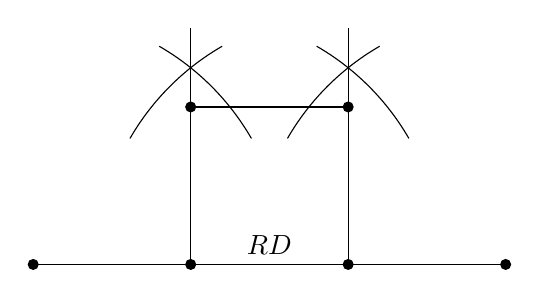
\begin{tikzpicture}
\draw (0,0) -- (6,0);
\foreach \i in {0,2,4,6}
  \fill (\i,0) circle (2pt);
\fill (2,2) circle (2pt);
\fill (4,2) circle (2pt);
\draw (2,2) -- (4,2);
\draw (2,0) -- (2,3);
\draw (4,0) -- (4,3);
\draw ([shift=(30:3.2cm)]0,0) arc (30:60:3.2cm);
\draw ([shift=(150:3.2cm)]4,0) arc (150:120:3.2cm);
\draw ([shift=(30:3.2cm)]2,0) arc (30:60:3.2cm);
\draw ([shift=(150:3.2cm)]6,0) arc (150:120:3.2cm);
\path (2,0) -- node[above] {$RD$} (4,0);
\end{tikzpicture}
\end{center}

\item \mbox{}
\[
\frac{355}{113}=3.14159292\,.
\]

\end{enumerate}

\selectlanguage{english}
%\hspace*{-5em}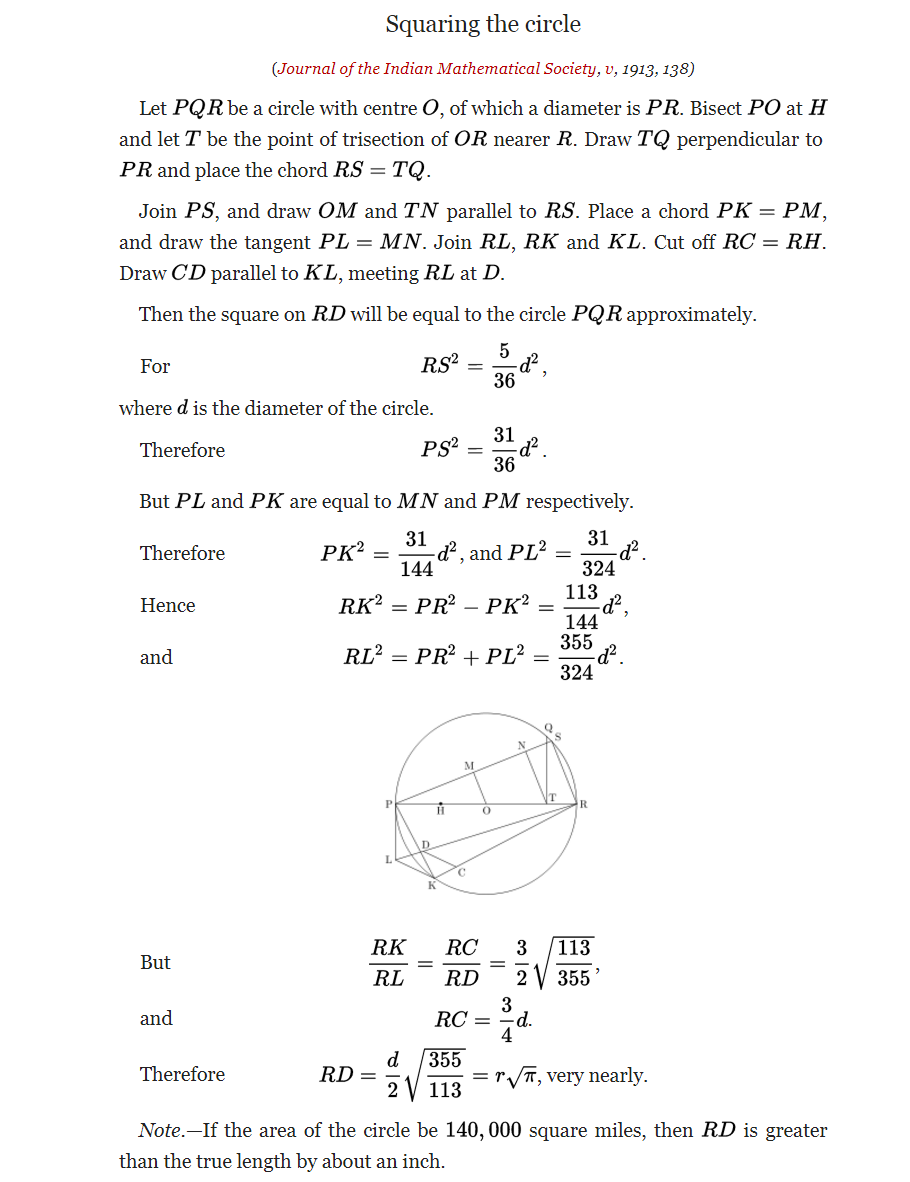
\includegraphics[width=1.2\textwidth]{ramanujan.png}
